\section{Anforderungsanalyse}

Um ein Migrationskonzept entwerfen zu können wird zuerst die existierenden Anwendung kurz beschrieben und untersucht und mithilfe einer Literaturrecherche die notwendigen Anforderungen an die Migration erarbeitet.

\subsection{Existierender Code}
Ziel der Anwendung ist das Einsammeln der Timesheets, in dem Projekt aktiver Mitarbeiter, aus einem Box Verzeichnis, das Überprüfen dieser und die anschließende Rechnungs- und Report Erstellung. Die Prozesse werden jeweils manuell über eine Konsoleneingabe gestartet. Im Box-Verzeichnis liegt ein Projektmanagement-File, welcher alle Mitarbeiter enthält, die jemals in dem Projekt gearbeitet haben und markiert, welche auch aktuell aktiv sind und dem Kunden in Rechnung gestellt werden können. In Abbildung \ref{fig:pmo_python} wird der Aufbau der ursprünglichen Anwendung dargestellt.

\begin{figure}[H]
    \centering
    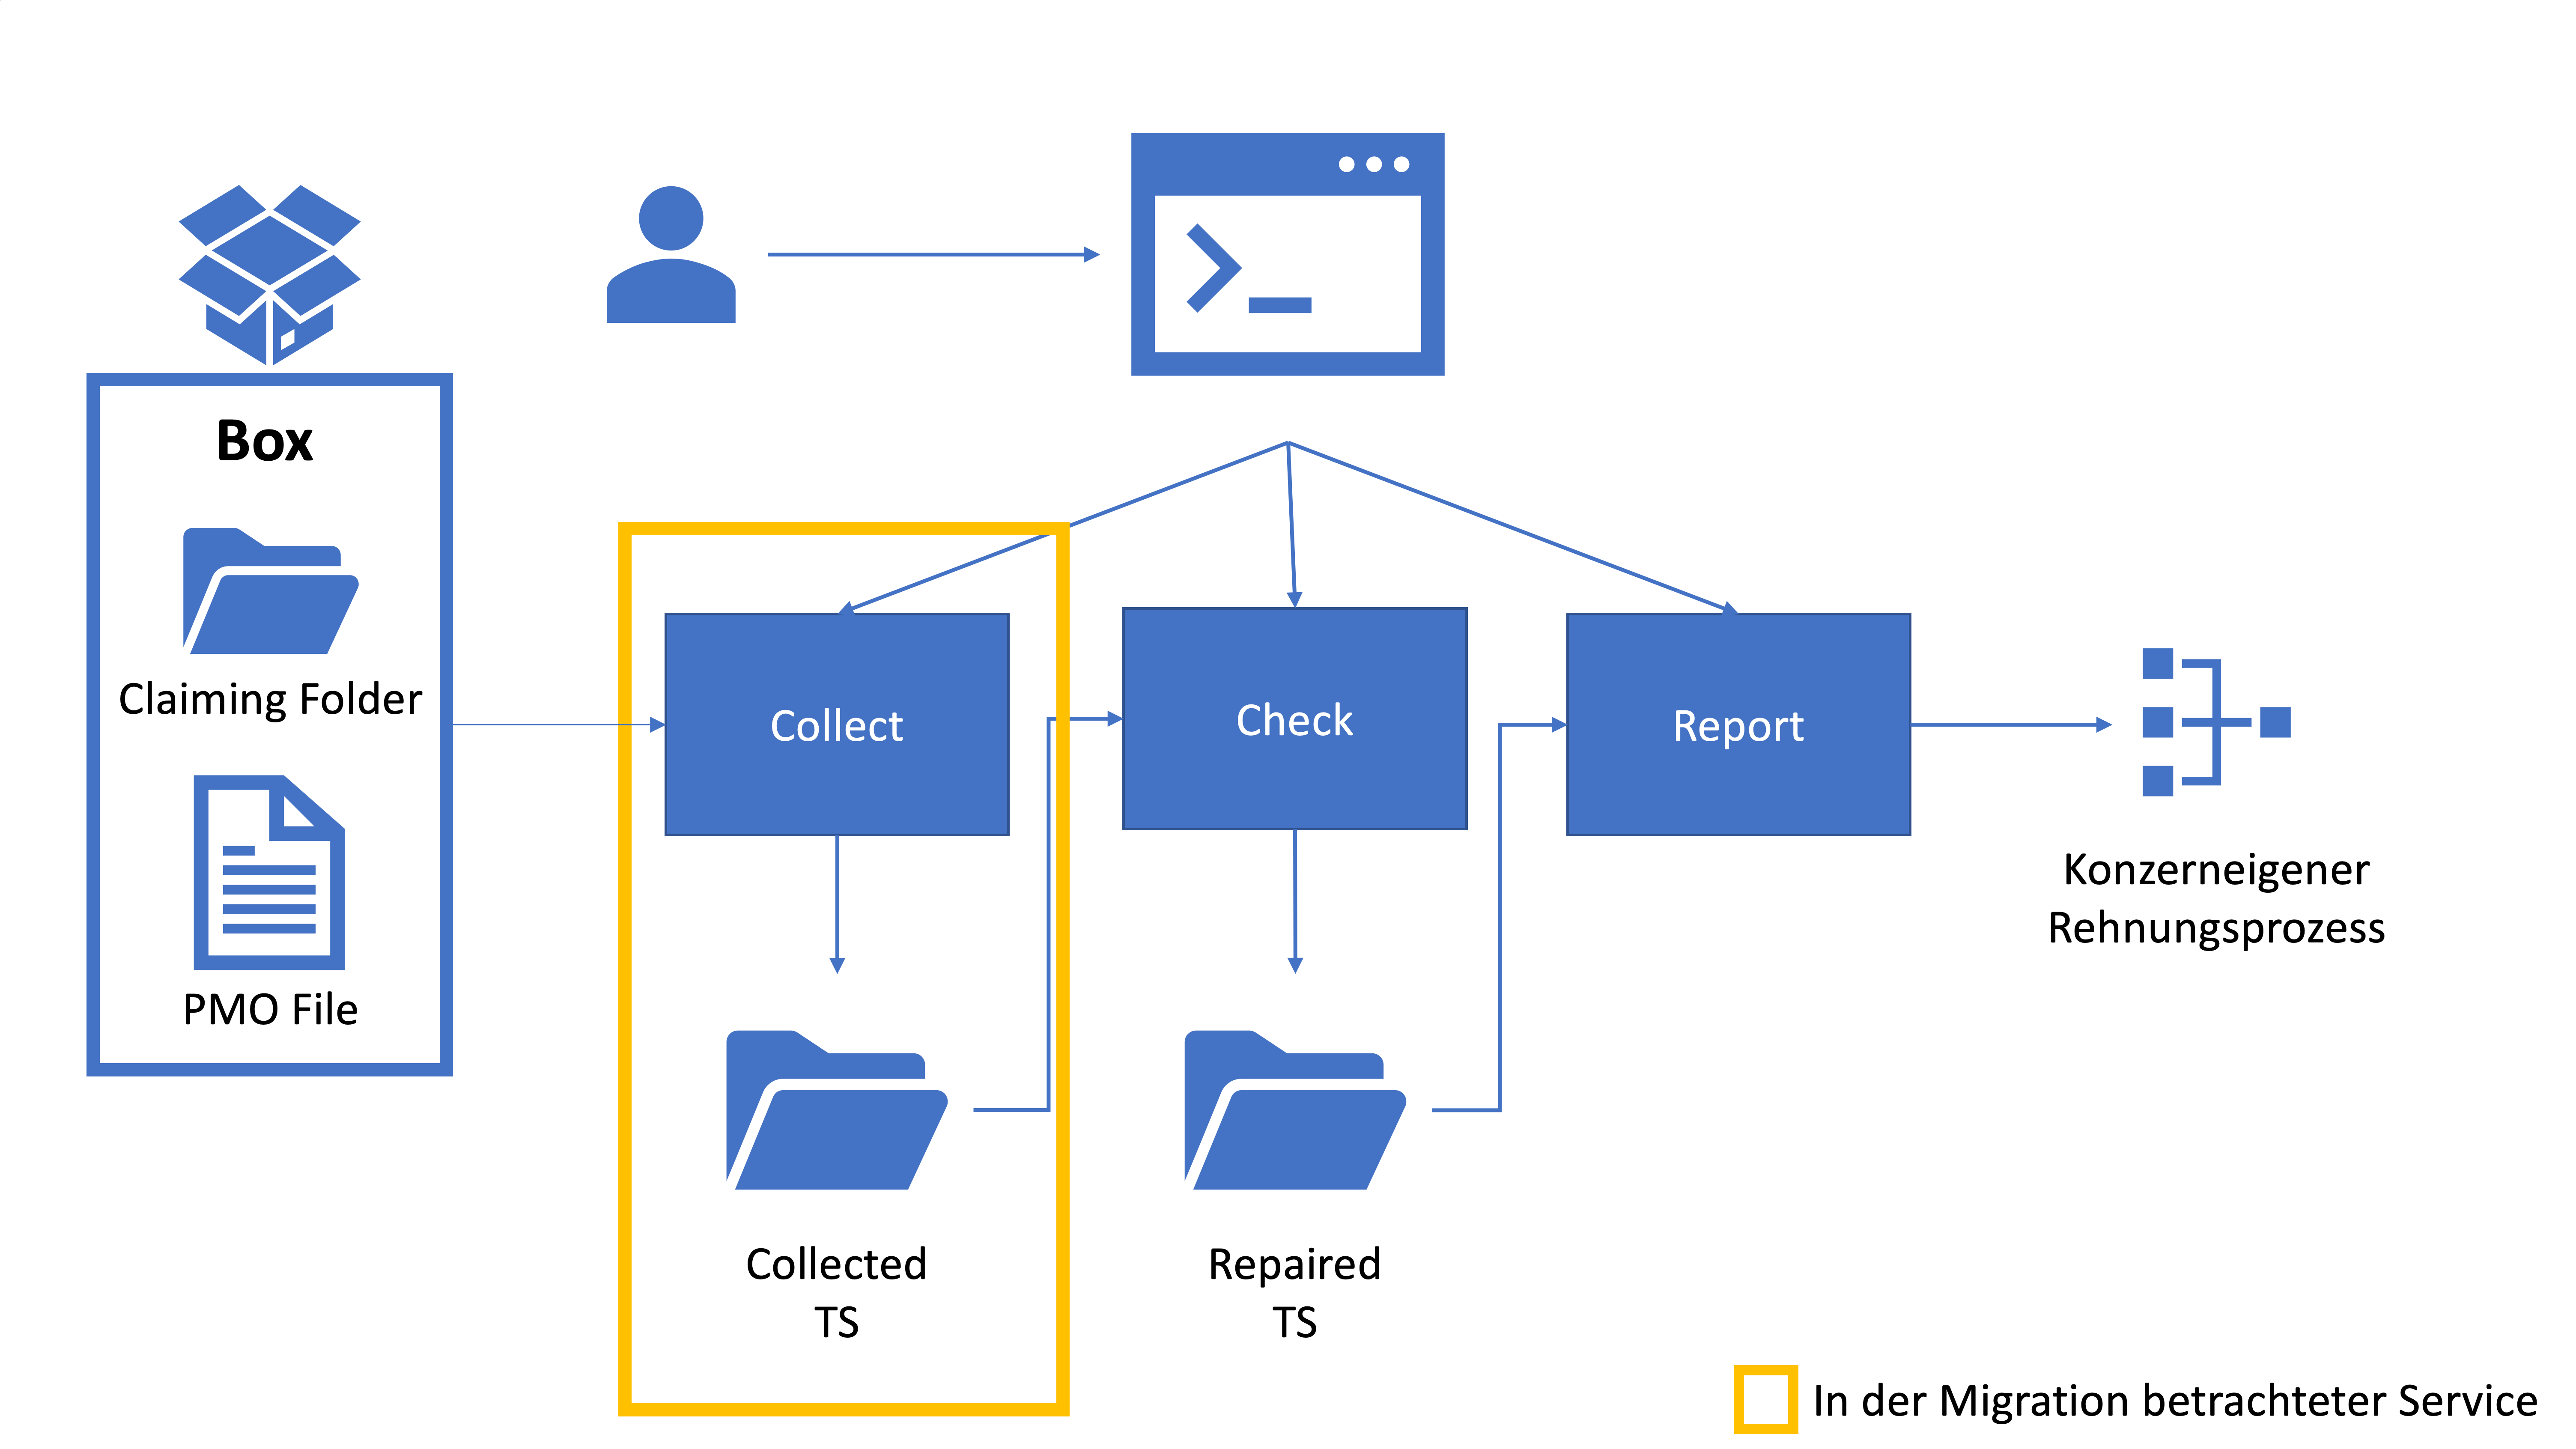
\includegraphics[width=0.65\textwidth]{pmo_python.png}
    \caption{Aufbau der ursprünglichen Anwendung (gelb umrandet der Teil, der prototypisch migriert wird)}
    \label{fig:pmo_python}
\end{figure}

Die bisher existierende Anwendung ist eine Python Anwendung, die grundsätzlich in dre Module aufgeteilt ist:
\begin{itemize}
\item \textbf{Timesheet Collector: }Einsammeln der Timesheets der in dem Projekt aktiven Mitarbeiter
\item \textbf{Timesheet Checker: }Überprüfen der Timesheets auf Korrektheit uns Vollständigkeit und gegebenenfalls Reparatur dieser
\item \textbf{Report Creator: }Erzeugung eines Reports und automatisierte Rechnungsstellung
\end{itemize}

Jeder dieser drei Services ist ein eigenes Python Modul. Diese greifen jeweils auf weitere Services wie einen Excel-Helper und Checking-Tools zurück.

Da es sich bei dieser Arbeit um eine Machbarkeitsstudie mit Erstellung eines Prototypen handelt, wird im ersten Schritt nur die Migration des Collect Service untersucht, bevor die anderen, komplexeren Services migriert werden. Dies ist in Abbildung \ref{fig:pmo_python} entsprechend durch den gelben Rahmen gekennzeichnet. Der Collect Service benötigt eine Verbindung zu dem Box-Verzeichnis und einen Ablageort für die \glqq{eingesammelten}\grqq{} Timesheets.

\subsection{Anforderungen an die Cloud Migration}
Wird eine Anwendung in die Cloud migriert werden unter anderem folgende Vorteile erwartet \cite[Vgl. auch im Folgenden][03:23-05:36min]{AWS2019}:
\begin{itemize}
\item Kostensenkung
\item Steigerung der Produktivität
\item Agilität in der Entwicklung
\end{itemize}

Darüber hinaus muss vor der Migration untersucht und festgelegt werden, welche der in Kapitel \ref{sec:migrationsansaetze} herausgearbeiteten Migrationsstrategien verfolgt werden soll \cite[Vgl.][10:38-13:23min]{AWS2019}. Jede dieser Strategien bietet ihre Vor- und Nachteile, weshalb diese Entscheidung individuell von der Anwendungsarchitektur und der Art der Benutzung abhängig ist.
\pagebreak